\section{Experiment Design}
\label{sec:experiment-design}

This experiment evaluates whether public online video feeds can be transformed
into persistent pseudonymous identity profiles without using direct facial
identification. The study is designed as a proof-of-concept pipeline: raw public
camera footage is converted into structured observations, observations are
linked into within-camera tracks, and tracks are compared across camera views to
estimate whether repeated observable patterns can support cross-camera
pseudonymous profiling.

\subsection{Research Question and Claim}
\label{subsec:research-question}

The research question is: should the general public be concerned with public
online cameras? The experiment addresses this question through the following
claim: public video feeds can support the creation of persistent pseudonymous
cyber identity profiles through repeated observable patterns, even without
direct facial identification. Accordingly, the experiment does not attempt to
name individuals, infer legal identities, or verify biometric identity. Instead,
it measures whether anonymous people in public video can be repeatedly detected,
tracked, and assigned persistent profile identifiers.

\subsection{Apparatus and Pipeline}
\label{subsec:apparatus-pipeline}

The apparatus consists of four public camera video sources, local frame
extraction scripts, a YOLOv8 object detector, a lightweight tracking module, and
visualization scripts. The pipeline is implemented in Python and shell scripts.
Frames are extracted from public video streams or local video files using
\texttt{ffmpeg}. Person detections are produced with the YOLOv8n model. The
pipeline then assigns local track identifiers within each camera and global
pseudonymous identifiers across cameras.

Figure~\ref{fig:pipeline-contact-sheet} shows representative frames from the
annotated output videos. These videos provide a visual record of how raw public
camera footage is converted into bounding boxes, track IDs, and global profile
IDs.

\begin{figure}[htbp]
    \centering
    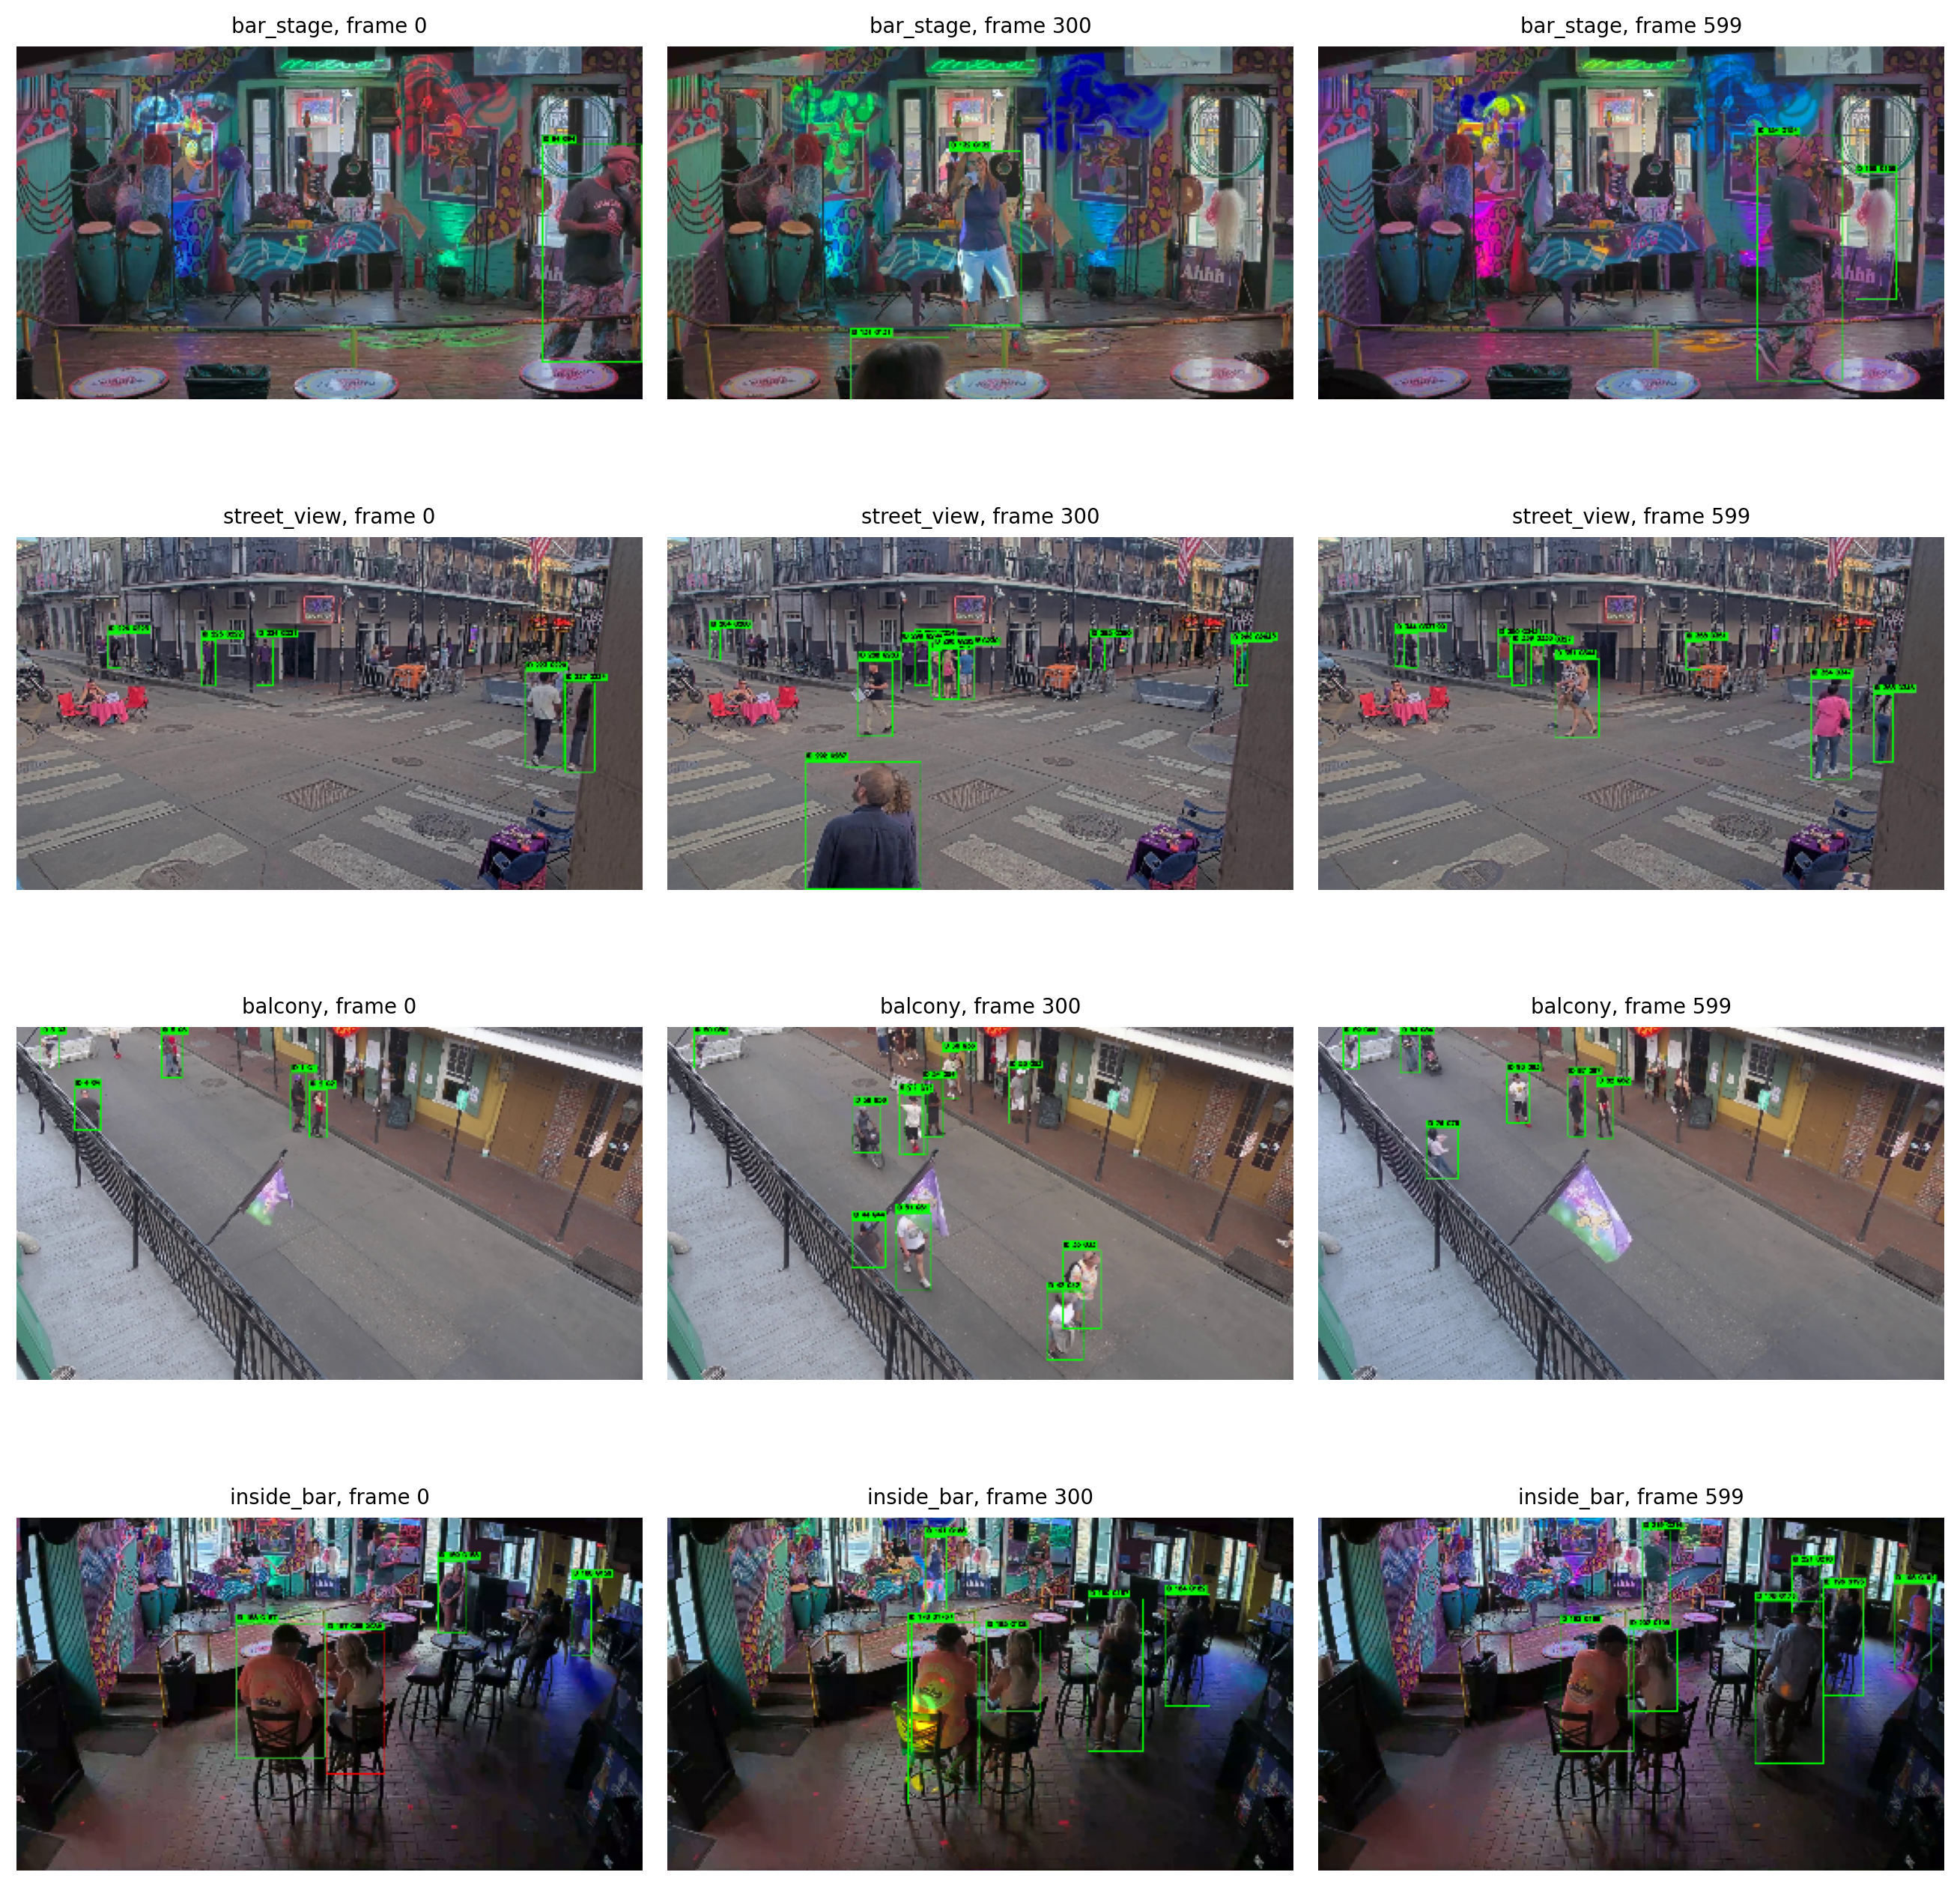
\includegraphics[width=\linewidth]{paper_figures/06_video_contact_sheet.png}
    \caption{Representative annotated frames from the output videos. Bounding
    boxes and profile labels illustrate how public camera footage is converted
    into structured observation records.}
    \label{fig:pipeline-contact-sheet}
\end{figure}

The pipeline has five stages:

\begin{enumerate}
    \item \textbf{Frame extraction.} Video frames are sampled from each public
    feed and stored by camera view.
    \item \textbf{Person detection.} YOLOv8n is applied to each frame, and only
    detections classified as \texttt{person} are retained.
    \item \textbf{Feature extraction.} For each detected person, the system
    extracts a simple appearance feature using HSV color histograms from the
    upper and lower regions of the detected body crop.
    \item \textbf{Within-camera tracking.} Consecutive detections in the same
    camera are linked using Hungarian assignment. The matching cost combines
    predicted center distance, bounding-box size difference, intersection over
    union, and appearance distance.
    \item \textbf{Cross-camera pseudonymous matching.} New track candidates are
    compared against global appearance profiles from other cameras. If the
    appearance distance is below the configured threshold, the detection is
    assigned to an existing global ID; otherwise, a new global ID is created.
\end{enumerate}

This design intentionally uses whole-person appearance features rather than
facial embeddings. As a result, the experiment focuses on identity-adjacent
profiling based on repeated observable patterns, not facial recognition.

\subsection{Dataset}
\label{subsec:dataset}

The evaluated dataset contains four camera views: balcony, bar stage, inside
bar, and street view. For each camera, the pipeline produced a detection CSV
file under \texttt{data/detections/}. Each CSV row represents one detected person
in one frame and includes the source camera, frame name, timestamp-like frame
index, bounding-box coordinates, detector confidence, local track ID, global
profile ID, and cross-camera match score when applicable.

The generated dataset also includes annotated videos for the four camera views:
\texttt{balcony.mp4}, \texttt{bar\_stage.mp4}, \texttt{inside\_bar.mp4}, and
\texttt{street\_view.mp4}. These videos were used as qualitative reference
material to confirm that the numerical outputs correspond to visible detections
and track labels in the frames.

\subsection{Evaluation Metrics}
\label{subsec:evaluation-metrics}

Because the purpose of the experiment is to evaluate feasibility rather than
biometric identification accuracy, the metrics are descriptive rather than
identity-ground-truth metrics. The primary metrics are:

\begin{itemize}
    \item \textbf{Detection volume:} the total number of person detections
    extracted from the public feeds.
    \item \textbf{Per-camera tracks:} the number of local track IDs generated
    within each camera view.
    \item \textbf{Global pseudonymous profiles:} the number of global IDs
    created by the cross-camera profile module.
    \item \textbf{Cross-camera profile span:} the number of distinct camera
    views in which each global ID appears.
    \item \textbf{Persistence:} the number of frames or detections associated
    with each global ID.
    \item \textbf{Detector confidence:} the YOLO confidence distribution by
    camera view.
    \item \textbf{Cross-camera match count:} the number of detections assigned a
    non-empty cross-camera match score.
\end{itemize}

These metrics are used to determine whether public video streams can be
converted into repeated, structured, and linkable observations. They should not
be interpreted as proof that the system can identify named individuals or as a
validated person re-identification benchmark.
